\documentclass{beamer}
\usetheme{metropolis}
\usepackage{graphicx}
\usepackage{subfig}
\usepackage{tcolorbox}
\title{Calculus-Based Physics-2: Electricity, Magnetism, and Thermodynamics (PHYS180-02): Unit 2}
\author{Jordan Hanson}
\institute{Whittier College Department of Physics and Astronomy}

\begin{document}
\maketitle

\section{Unit 1 Review}

\begin{frame}{Unit 1 Summary}
\textbf{Reading: Chapters 1 and 2}
\begin{enumerate}
\item Temperature, Heat, and the 0th Law of Thermodynamics
\item Heat flow and transfer mechanisms
\item Kinetic Theory of Gases
\end{enumerate}
\end{frame}

\begin{frame}{Unit 1 Review Problems}
\small
James Prescott Joule first published in December 1840, an abstract in the Proceedings of the Royal Society, suggesting that heat could be generated by an electrical current. Joule immersed a length of wire in a fixed mass of water and measured the temperature rise due to a known current flowing through the wire for a 30 minute period. By varying the current and the length of the wire he deduced that the heat produced was proportional to the square of the current multiplied by the electrical resistance of the immersed wire. \\ \vspace{0.5cm} Wikipedia: \url{https://en.wikipedia.org/wiki/Joule_heating}.
\end{frame}

\begin{frame}{Unit 1 Review Problems}
Suppose the wire of J. Joule is carrying 10 W of power.  If the mass of the water in the container is 1 kg, how long will it take to raise the temperature of the water by 5 degrees?  (The heat capacity of water is 4186 J/kg/$^{\circ}$C).
\begin{itemize}
\item A: 10 seconds
\item B: 80 seconds
\item C: 420 seconds
\item D: 3600 seconds
\end{itemize}
\end{frame}

\begin{frame}{Unit 1 Review Problems}
Suppose the the water begins at 95 $^{\circ}$C, and ends at 100 $^{\circ}$C.  How long will it take to boil away all of the water?  (The latent heat of vaporization of water is 2256 kJ/kg).
\begin{itemize}
\item A: About an hour
\item B: About 6 hours
\item C: About 60 hours
\item D: Several days
\end{itemize}
\end{frame}

\begin{frame}{Unit 1 Review Problems}
\begin{figure}
\centering
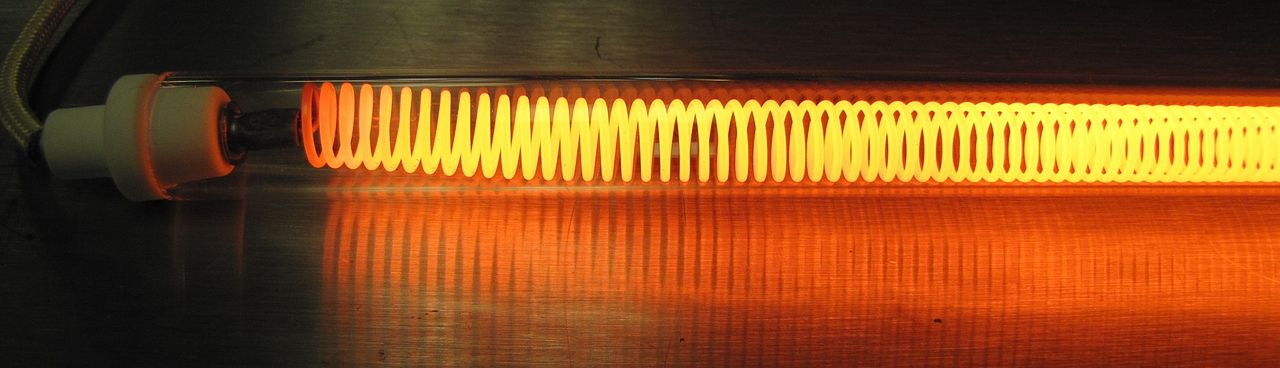
\includegraphics[width=0.9\textwidth]{figures/toaster.JPG}
\caption{\label{fig:toast} An example of Joule heating in a toaster coupling.}
\end{figure}
\end{frame}

\section{Summary}

\begin{frame}{Unit 1 Summary}
\textbf{Reading: Chapters 3 and 4}
\begin{enumerate}
\item The First Law of Thermodynamics
\item The Second Law of Thermodynamics
\end{enumerate}
\end{frame}

\section{JITT - Reading Quiz Results}

\section{The First Law of Thermodynamics}

\begin{frame}{The First Law of Thermodynamics}
\alert{Equation of state}: The equation of state of a system, in general, looks like this:
\begin{equation}
f(p,V,T) = 0
\end{equation}
\begin{itemize}
\item $V$ is an \textbf{extensive} variable.
\item $p$ and $V$ are \textbf{intensive} variables.
\item Holding \textit{intensive} variables constant, doubling the mass of a system doubles the volume.  That is the relationship between intensive and extensive variables.
\end{itemize}
\end{frame}

\begin{frame}{The First Law of Thermodynamics}
\alert{The equation of state of an ideal gas} looks like this:
\begin{equation}
pV - nRT = 0
\end{equation}
Which of the following is correct?
\begin{itemize}
\item A: The extensive variables are $p$, $V$, and $R$
\item B: The only extensive variable is $n$, and $p$, $V$, and $T$ are the intensive ones
\item C: The only extensive variable is $n$, and $p$ is the only intensive one
\item D: There are no extensive variables because none of them is mass
\end{itemize}
\end{frame}

\begin{frame}{The First Law of Thermodynamics}
Recall that the definition of work done on a system is:
\begin{equation}
W = \int \vec{F} \cdot d\vec{x}
\label{eq:work}
\end{equation}
\begin{itemize}
\item $\vec{F}$ is the net force acting on the system
\item $d\vec{x}$ is the incremental displacement
\end{itemize}
\end{frame}

\begin{frame}{The First Law of Thermodynamics}
Example: suppose the force is gravity, near the surface of the Earth $\vec{F} = -mg \hat{y}$, and an object at height $h$ is released.
\begin{equation}
W = \int \vec{F} \cdot d\vec{x} = -mg \hat{y} \cdot -h\hat{y} = mgh
\label{eq:work2}
\end{equation}
\begin{itemize}
\item $\vec{F}$ is the net force acting on the system
\item $d\vec{x}$ is the incremental displacement
\item Work-energy theorem can give the final speed: $\frac{1}{2}mv_{\rm f}^2 = mgh$.
\end{itemize}
\end{frame}

\begin{frame}{The First Law of Thermodynamics}
Definition of work, applied to a thermodynamic system \textit{with an equation of state}:
\begin{equation}
W = \int \vec{F} \cdot d\vec{x} = \int p\vec{A} \cdot d\vec{x} = \int p dV
\label{eq:work3}
\end{equation}
\begin{itemize}
\item $\vec{A}$ and $d\vec{x}$ assumed to be parallel
\item $p$ is constant over $d\vec{x}$
\end{itemize}
\end{frame}

\begin{frame}{The First Law of Thermodynamics}
Definition of work, applied to a thermodynamic system \textit{with an equation of state}:
\begin{equation}
W = \int p dV
\label{eq:work4}
\end{equation}
\textbf{Group board exercise:} Substitute the Ideal Gas Law into Eq. \ref{eq:work4}, to derive the work done \textit{when temperature is constant and $V$ is the independent variable}. \\ \vspace{0.5cm}
\textit{Hint: the integral of $\frac{1}{x}$ is $\ln x + C$.} \\
\vspace{0.5cm}
\textbf{Group board exercise:} Repeat, but at \textit{constant pressure} instead of constant temperature, again with $V$ as the independent variable.
\end{frame}

\begin{frame}{The First Law of Thermodynamics}
The van der Waals \textit{equation of state} is: 
\begin{equation}
\left(p+\frac{a}{V^2}\right)\left(V-b\right) - nRT = 0
\label{eq:vanDerWaals}
\end{equation}
\textbf{Group board exercise:} Substitute this equation of state into Eq. \ref{eq:work4}, to find the work done by isothermal expansion.  Compare to the isothermal result from the Idea Gas Law, and recover the previous result for $W$ by setting $a$ and $b$ to zero.
\end{frame}

\begin{frame}{The First Law of Thermodynamics}
\begin{figure}
\centering
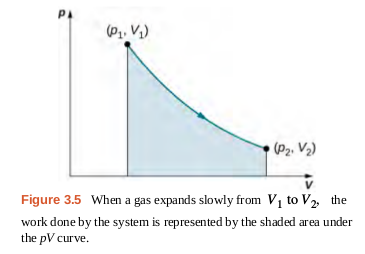
\includegraphics[width=0.45\textwidth]{figures/area1.png}
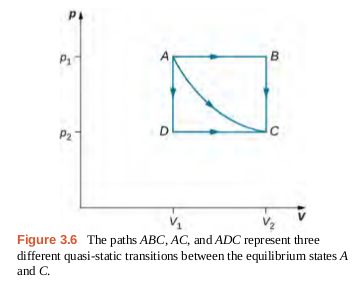
\includegraphics[width=0.45\textwidth]{figures/area2.png}
\caption{\label{fig:area} \small On a $pV$ diagram, work is the area under the curve, in the same fashion that it is the area under the curve on a force displacement diagram.}
\end{figure}
\end{frame}

\begin{frame}{The First Law of Thermodynamics}
How much energy is available to do work, in the form of heat?  (For example, if we expand a gas at constant pressure, by how much can we decrease the temperature?) \\ \vspace{0.5cm}
Recall from the prior chapter that 
\begin{equation}
\boxed{
E_{\rm int} = \frac{3}{2}nRT = \frac{3}{2}nN_{\rm A}k_{\rm B}T = \frac{3}{2}NkT}
\label{eq:internal}
\end{equation}
The \textit{internal energy} of a gas must be comprised of the average kinetic energies of the molecules.  Here we ignore molecular interactions.
\end{frame}

\begin{frame}{The First Law of Thermodynamics}
\begin{tcolorbox}[colback=white,colframe=red!40!blue,title=The First Law of Thermodynamics]
\alert{Associated with every equilibrium state of a system is its internal energy $E_{\rm int}$.  The change in $E_{\rm int}$ for any transition between two equilibrium states is $\Delta E_{\rm int} = Q-W$, where $Q$ is the heat exchanged by the system and $W$ is the work done on or by the system.}
\end{tcolorbox}
\begin{itemize}
\item If heat is added to the system: $Q>0$
\item If heat is removed from the system: $Q<0$
\item If work is done by the system: $W>0$
\item If work is done on the system: $W<0$
\end{itemize}
\end{frame}

\begin{frame}{The First Law of Thermodynamics}
In each of the following scenarios, select the best answer:
\small
\begin{itemize}
\item A: $E_{\rm int}$ increases
\item B: $E_{\rm int}$ decreases
\item C: $E_{\rm int}$ does not change
\item D: I am confused.
\end{itemize}
\small
\begin{itemize}
\item Scenario 1: \alert{A gas expands against a piston, doing some work, but the gas loses no heat.}
\item Scenario 2: A gas expands against a piston, performing 10 J of work.  A separate device adds 10 J of heat to the gas.
\item Scenario 3: A piston is pushed against a gas, requiring 10 J of work.  A separate device adds 10 J of heat to the gas.
\end{itemize}
\end{frame}

\begin{frame}{The First Law of Thermodynamics}
In each of the following scenarios, select the best answer:
\small
\begin{itemize}
\item A: $E_{\rm int}$ increases
\item B: $E_{\rm int}$ decreases
\item C: $E_{\rm int}$ does not change
\item D: I am confused.
\end{itemize}
\small
\begin{itemize}
\item Scenario 1: A gas expands against a piston, doing some work, but the gas loses no heat.
\item Scenario 2: \alert{A gas expands against a piston, performing 10 J of work.  A separate device adds 10 J of heat to the gas.}
\item Scenario 3: A piston is pushed against a gas, requiring 10 J of work.  A separate device adds 10 J of heat to the gas.
\end{itemize}
\end{frame}

\begin{frame}{The First Law of Thermodynamics}
In each of the following scenarios, select the best answer:
\small
\begin{itemize}
\item A: $E_{\rm int}$ increases
\item B: $E_{\rm int}$ decreases
\item C: $E_{\rm int}$ does not change
\item D: I am confused.
\end{itemize}
\small
\begin{itemize}
\item Scenario 1: A gas expands against a piston, doing some work, but the gas loses no heat.
\item Scenario 2: A gas expands against a piston, performing 10 J of work.  A separate device adds 10 J of heat to the gas.
\item Scenario 3: \alert{A piston is pushed against a gas, requiring 10 J of work.  A separate device adds 10 J of heat to the gas.}
\end{itemize}
\end{frame}

\begin{frame}{The First Law of Thermodynamics}
In each of the following scenarios, select the best answer:
\small
\begin{itemize}
\item A: $E_{\rm int}$ increases
\item B: $E_{\rm int}$ decreases
\item C: $E_{\rm int}$ does not change
\item D: I am confused.
\end{itemize}
\small
\begin{itemize}
\item Scenario 4: \alert{A cold scientist clutches a warm canteen of water to his chest (the system is the canteen).}
\item Scenario 5: A cylinder of gas has a piston on one end.  Someone pulls the piston slowly, doing 10 J of work.
\end{itemize}
\end{frame}

\begin{frame}{The First Law of Thermodynamics}
In each of the following scenarios, select the best answer:
\small
\begin{itemize}
\item A: $E_{\rm int}$ increases
\item B: $E_{\rm int}$ decreases
\item C: $E_{\rm int}$ does not change
\item D: I am confused.
\end{itemize}
\small
\begin{itemize}
\item Scenario 4: A cold scientist clutches a warm canteen of water to his chest (the system is the canteen).
\item Scenario 5: \alert{A cylinder of gas has a piston on one end.  Someone pulls the piston slowly, doing 10 J of work.}
\end{itemize}
\end{frame}

\begin{frame}{The First Law of Thermodynamics}
\begin{figure}
\centering
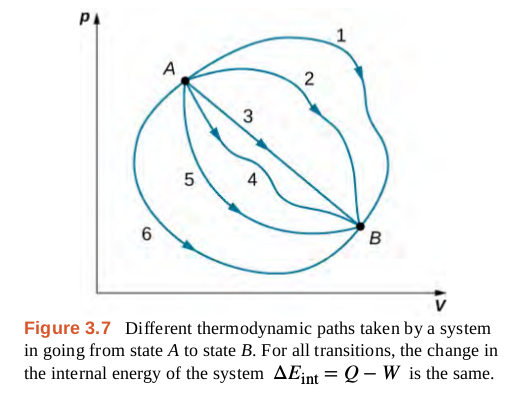
\includegraphics[width=0.6\textwidth]{figures/states1.png}
\caption{\label{fig:states} The internal energy for a given state depends only on the temperature, and not the path taken to arrive at that state.}
\end{figure}
\end{frame}

\begin{frame}{The First Law of Thermodynamics}
\begin{columns}[T]
\begin{column}{0.5\textwidth}
\small Which of the following is true of the \textit{work done by the system}?
\begin{itemize}
\item A: Path 2 corresponds to the most work done, and path 5 the least work done.
\item B: Path 5 corresponds to the most work done, and path 2 the least work done.
\item C: Path 3 corresponds to the most work done, and path 4 the least work done.
\item D: Path 4 corresponds to the most work done, and path 3 the least work done.
\end{itemize}
\end{column}
\begin{column}{0.5\textwidth}
\begin{figure}
\centering
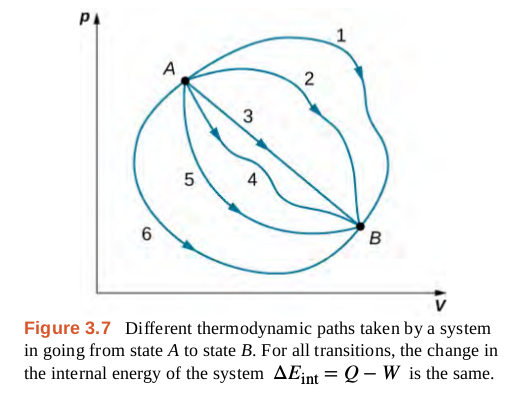
\includegraphics[width=\textwidth]{figures/states1.png}
\caption{\label{fig:states2} Use this diagram to answer the questions at left}
\end{figure}
\end{column}
\end{columns}
\end{frame}

\begin{frame}{The First Law of Thermodynamics}
\begin{columns}[T]
\begin{column}{0.5\textwidth}
\small Suppose $\Delta E_{\rm int} = 0$.  Which of the following is true?
\begin{itemize}
\item A: For path 1, the system gains the most heat.
\item B: For path 5, the system loses the most heat.
\item C: For path 3, the system loses the most heat.
\item D: For path 1, the system loses the most heat.
\end{itemize}
\end{column}
\begin{column}{0.5\textwidth}
\begin{figure}
\centering
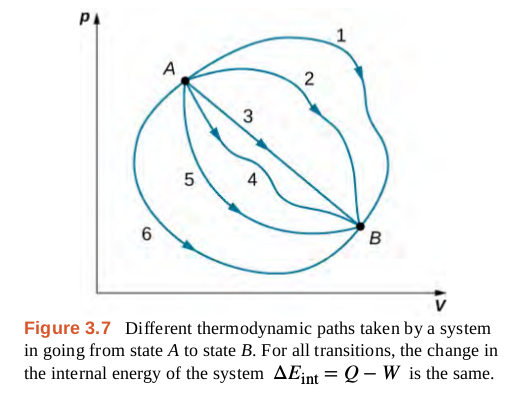
\includegraphics[width=\textwidth]{figures/states1.png}
\caption{\label{fig:states3} Use this diagram to answer the questions at left}
\end{figure}
\end{column}
\end{columns}
\end{frame}

\begin{frame}{The First Law of Thermodynamics}
\begin{columns}[T]
\begin{column}{0.5\textwidth}
\small Suppose the system in question is an ideal gas.  Which path most likely represents a transition with constant temperature?
\begin{itemize}
\item A: Path 3
\item B: Path 2
\item C: Path 5
\item D: Path 1
\end{itemize}
\end{column}
\begin{column}{0.5\textwidth}
\begin{figure}
\centering
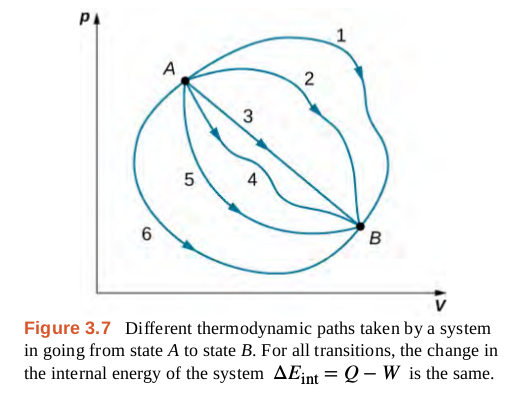
\includegraphics[width=\textwidth]{figures/states1.png}
\caption{\label{fig:states4} Use this diagram to answer the questions at left}
\end{figure}
\end{column}
\end{columns}
\end{frame}

\begin{frame}{The First Law of Thermodynamics}
Recall that the work done by an $n$ moles of an expanding ideal gas at constant temperature $T$ is given by $W = nRT\ln(V_{\rm f}/V_{\rm i})$, where $R = 8.314$ J/mole/Kelvin.  Calculate the work done if heat is added to 2 moles of an ideal gas at 300 K such that the volume of the gas grows by a factor of 2.
\begin{itemize}
\item A: 416 J
\item B: 520 J
\item C: 3460 J
\item D: 4320 J
\end{itemize} 
\end{frame}

\begin{frame}{The First Law of Thermodynamics}
Same scenario, but calculate the work if the gas was at a constant temperature of 200 K.
\begin{itemize}
\item A: 2305 J
\item B: 3410 J
\item C: 280 J
\item D: 320 J
\end{itemize} 
\end{frame}

\begin{frame}{The First Law of Thermodynamics}
If the temperature remains at 200K during the process, what is the heat transferred into or out of the system?
\begin{itemize}
\item A: -2305 J
\item B: 2305 J
\item C: -3410 J
\item D: 3410 J
\end{itemize} 
\end{frame}

\begin{frame}{The First Law of Thermodynamics}
Suppose we have a system where we can add external heat into a rocket, and then 100 percent of that heat is converted to kinetic energy for the rocket.  If the rocket has 0.1 kg of mass, and $g = 10$ m/s/s, how much heat is required to launch the rocket to a height of 50 meters?
\begin{itemize}
\item A: 20 J
\item B: 30 J
\item C: 40 J
\item D: 50 J
\end{itemize} 
\end{frame}

\begin{frame}{The First Law of Thermodynamics}
If in the heat-to-rocket system, we have to provide the heat first to 2 moles of an ideal gas, what would be the required temperature change?
\begin{itemize}
\item A: 2 degrees C
\item B: 3 degrees C
\item C: 20 degrees C
\item D: 30 degrees C
\end{itemize} 
\end{frame}

\begin{frame}{The First Law of Thermodynamics}
In the previous two problems we equated heat energy with mechanical energy: $mgh = Q$, and then calculated $Q$ with $Q=\frac{3}{2}nRT$.  Thus, we used $mgh = \frac{3}{2}nRT$.  Let's try one with kinetic energy instead of potential energy. \\ \vspace{0.5cm}
If we are using the heat stored in 2 moles of an ideal gas, what temperature change is required to get that heat to accelerate a 0.1 kg object to 10 m/s?
\begin{itemize}
\item A: 3 degrees C
\item B: 2 degrees C
\item C: 0.3 degrees C
\item D: 0.2 degrees C
\end{itemize} 
\end{frame}

\begin{frame}{The First Law of Thermodynamics}
\begin{figure}
\centering
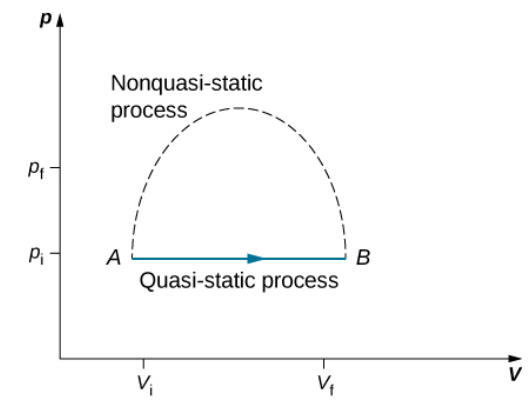
\includegraphics[width=0.5\textwidth]{figures/process.png}
\caption{\label{fig:process} Two processes: quasi-static and non-quasi-static.  We study state transitions composed of many quasi-static transitions.  The pictured non-quasi-static transition has two volumes with the same pressure, so how can we reasonably define the state of a system?}
\end{figure} 
\end{frame}

\begin{frame}{The First Law of Thermodynamics}
Words of the text: ``A quasi-static transition is one in which the change in state is made infinitesimally slowly so that at each instant, the system can be assumed to be at a thermodynamic equilibrium with itself and with the environment.'' \\ \vspace{0.5cm}
\textbf{What follows are a few examples of thermodynamic processes that may be classified as quasi-static.} In realistic systems, some amount of non-quasi-static behavior is normal.
\end{frame}

\begin{frame}{The First Law of Thermodynamics}
A process is called \textbf{cyclic} if it returns a system to the same state with the same internal energy.
We should know at least these types of quasi-static processes: \small 
\begin{enumerate}
\item Isothermal ($T$ is constant)
\item Isobaric ($p$ is constant)
\item Adiabatic ($Q$, the head added/subtracted, is zero)
\item Isochoric ($V$ is constant)
\end{enumerate}
Exercise: use the following simulation to create cyclic processes.
\url{https://www.geogebra.org/m/mXvUPjFz}
\end{frame}

\begin{frame}{The First Law of Thermodynamics}
Exercise: use the following simulation to create cyclic processes: \url{https://www.geogebra.org/m/mXvUPjFz}.  What do you notice about the total heat exchanged $Q$, and the total work done, $W$?
\begin{enumerate}
\item Create four different cyclic processes that involve the four quasi-static process types, and explain quantitatively (in your lab notebook) why each fits the relevant criterion.
\item What is true about $Q$ and $W$ for each of these for processes you've created?  Why is this the case?
\end{enumerate}
\end{frame}

\section{Heat Capacities of an Ideal Gas}

\begin{frame}{Heat Capacities of an Ideal Gas}
\small What follows is a traditional proof of the following theorem:
\begin{equation}
C_{\rm P} = C_{\rm V} + R
\end{equation}
\textit{The molar heat capacity of a gas at constant pressure is always larger than at constant volume.} \\ \vspace{0.5cm}
\begin{itemize}
\item \textbf{Assume} an ideal gas
\item \textbf{Apply} First Law of Thermodynamics
\item Evidence for \textit{independence of state function}
\item Evidence for \textit{kinetic theory of gases}
\end{itemize}
\end{frame}

\begin{frame}{Heat Capacities of an Idea Gas}
\small
The first law of thermodynamics: $dE = dQ - dW$.  Consider an ideal gas, in a vessel with fixed volume.  Since $dW = pdV$, $dW=0$.  If heat $dQ$ is added to that vessel, the corresponding temperature in increase is
\begin{equation}
dQ = n C_{\rm V} dT
\end{equation}
where $C_{\rm V}$ represents the \textit{heat capacity at constant volume} \footnote{Recall that from kinetic theory, for ideal gases with no molecular interactions, $C_{\rm V} = \frac{3}{2}R$.}.  Because $dE = dQ$,
\begin{equation}
dE = n C_{\rm V} dT
\end{equation}
\end{frame}

\begin{frame}{Heat Capacities of an Idea Gas}
\small
Consider the same gas, but at fixed pressure.  Beginning with first law of thermodynamics now accounts for work: \\ $dE = dQ - dW = dQ - pdV$.  If heat $dQ$ is added to the vessel, the corresponding temperature change is
\begin{equation}
dQ = n C_{\rm P} dT \label{eq:dq}
\end{equation}
where $C_{\rm P}$ is the \textit{heat capacity at constant pressure.}  In order to obtain an expression for $dE$ involving only temperature, the ideal gas law must be differentiated:
\begin{align}
d(pV) &= d(nRT) \\
pdV &= nRdT \label{eq:pdv}
\end{align}
Substituting the right-hand side of Eq. \ref{eq:pdv} for $dW$ in the First Law, and the right-hand side of Eq. \ref{eq:dq} for $dQ$ in the first law, the result is
\begin{equation}
dE = n(C_{\rm P} - R)dT
\end{equation}
\end{frame}

\begin{frame}{Heat Capacities of an Idea Gas}
The expressions for $dE$ under isobaric and isochoric conditions have been obtained:
\begin{align}
dE &= C_{\rm V} dT \\
dE &= n(C_{\rm P} - R)dT
\end{align}
If the internal energy of a thermodynamic system depends only on the temperature, then these two expressions must be equal.  Upon setting them equal, a fundamental relationship is revealed:
\begin{equation}
\boxed{
C_{\rm P} = C_{\rm V} + R}
\end{equation}
It has been shown that $C_{\rm V} = \frac{3}{2}R$ from the equipartition principle, so $C_{\rm P} = \frac{5}{2}R$ for an ideal gas.
\end{frame}

\begin{frame}{Heat Capacities of an Ideal Gas}
\small
Jasmine, the heroine of \textit{Artemis}, by Andy Weir, lives on the moon.  Suppose she needs to power up a bulkhead in a compartment that has lost pressure, but the bulkhead won't work below a certain temperature.  She devises a plan fill up a heated container with oxygen and open it in the compartment, both releasing oxygen and heat.  How should she fill the container with heated air, to store the most heat in a given time limit?
\begin{itemize}
\item A: Fill a fixed-volume container with low-pressure air and heat it up.
\item B: Fill an inflatable object with heated air at constant, low pressure.
\item C: Fill a fixed-volume object with high-pressure air and heat it up.
\item D: Fill an inflatable object with heated air at high pressure.
\end{itemize}
\end{frame}

\begin{frame}{Heat Capacities of an Ideal Gas}
\small
\begin{itemize}
\item A: Fill a fixed-volume container with low-pressure air and heat it up.
\item B: Fill an inflatable object with heated air at constant, low pressure.
\item C: Fill a fixed-volume object with high-pressure air and heat it up.
\item D: Fill an inflatable object with heated air at high pressure.
\end{itemize}
\textit{I would say \textbf{D}, merely because we know that the heat capacity of the gas is higher at constant pressure rather than constant volume, and at high pressure we get more atoms of gas...}
\end{frame}

\section{Adiabatic Processes with an Ideal Gas}

\section{Conclusion}

\section{Answers}

\begin{frame}{Answers}
\small
\begin{columns}[T]
\begin{column}{0.5\textwidth}
\begin{itemize}
\item 420 seconds
\item About 60 hours
\item The only extensive variable is $n$, and $p$, $V$, and $T$ are the intensive ones
\item $E_{\rm int}$ decreases
\item $E_{\rm int}$ does not change
\item $E_{\rm int}$ increases
\item $E_{\rm int}$ decreases
\item Path 5
\item 3460 J
\end{itemize}
\end{column}
\begin{column}{0.5\textwidth}
\begin{itemize}
\item 2305 J
\item -2305 J
\item 50 J
\item 0.2 degrees C
\item Fill an inflatable object with heated air at high pressure.
\end{itemize}
\end{column}
\end{columns}
\end{frame}

\end{document}
